\chapter{Analysis of Breakpoint Features in Evolutionary and Cancer Contexts}
\label{chap_breakpoint_analysis}
It is important not only to be able to locate genomic breakpoints, but also to understand the genomic contexts in which they are located. This can give insights into the mechanisms of their formation, and to their impact on genome structure and function. As mentioned previously, evolutionary breakpoints that break synteny between species have parallels in the genomic breakpoints that occur within cancer cells: at some point in time SVs created these breakpoints, which were then conserved through evolutionary history. One especially interesting example can be found in the genome of the gibbon, which has many more genomic rearrangements with respect to the other apes than would be expected given their degree of relatedness.

\section{Evolutionary Breakpoints in the Gibbon Genome determined by BACs}

To search for genomic features potentially associated with gibbon chromosomal breakpoints I computed the significance of the overlap between gibbon evolutionary breakpoint regions, which had been identified and mapped to the human genome using bacterial artificial chromosomes (BACs) and array painting, and a set of genomic features of interest using permutation tests~\cite{Capozzi:2012bb}. The purpose of the permutation analysis is to discover the null distribution for the number of overlaps a set of intervals has with a particular feature in the genome. In essence, the test asks: if my intervals were placed in random locations on the genome, what is the probability of seeing the number of overlaps we observed with that features in the actual data? 

To conduct the test, while maintaining the chromosomal assignment and length of break- point regions, we permuted their start coordinates 10,000 times using BEDTools version 2.16.2~\cite{Quinlan:2010km}. Genomic regions annotated as centromeres and telomeres in the ``Gaps'' track of the hg19 build were excluded from possible random placements of the regions. Locations of the features were held constant. We then compared the number of features that overlapped a breakpoint region to the observed distribution of results among the randomly permuted regions, and used the quantile of the real observed value in that distribution as an estimate of the P-value of observing a value equal to or greater than the real observation. In order to be able to conduct a large number of permutations to determine a true background distribution for each feature, I have created a pipeline for distributing computation across a compute cluster using the grid management system HTCondor.

The analysis was performed on the human hg19 assembly. The features examined were genes, human segmental duplications, and some repeat families (Alu, LINE, ERV, and SVA). We also investigated the associations between breakpoint regions and chromatin structure by testing the overlap with open chromatin regions in human embryonic stem cells reported by the ENCODE consortium~\cite{ENCODEProjectConsortium:2011iz}. We found a significant enrichment for genes (Bonferroni adjusted P-value = 0.0287), human segmental duplications (P = 0.0366), Alu (P < 0.0001), and SVA (P = 0.0008) (Fig.~\ref{gibbon_bac_permutations}A). We did not find significant enrichment for LINE and ERV repeats, nor for the ENCODE open chromatin regions. Systematically shifting the location of breakpoint regions by increments of 10 kb up- and downstream of their actual location, up to a maximum of 1 MB, shows that the locations of the breakpoint regions gives the greatest or close to the greatest number of overlaps with the four significantly overlapping features (genes, segmental duplications, Alu, and SVA) in the local genomic neighborhood (Fig.~\ref{gibbon_bac_permutations}B).

\begin{figure}
\centering
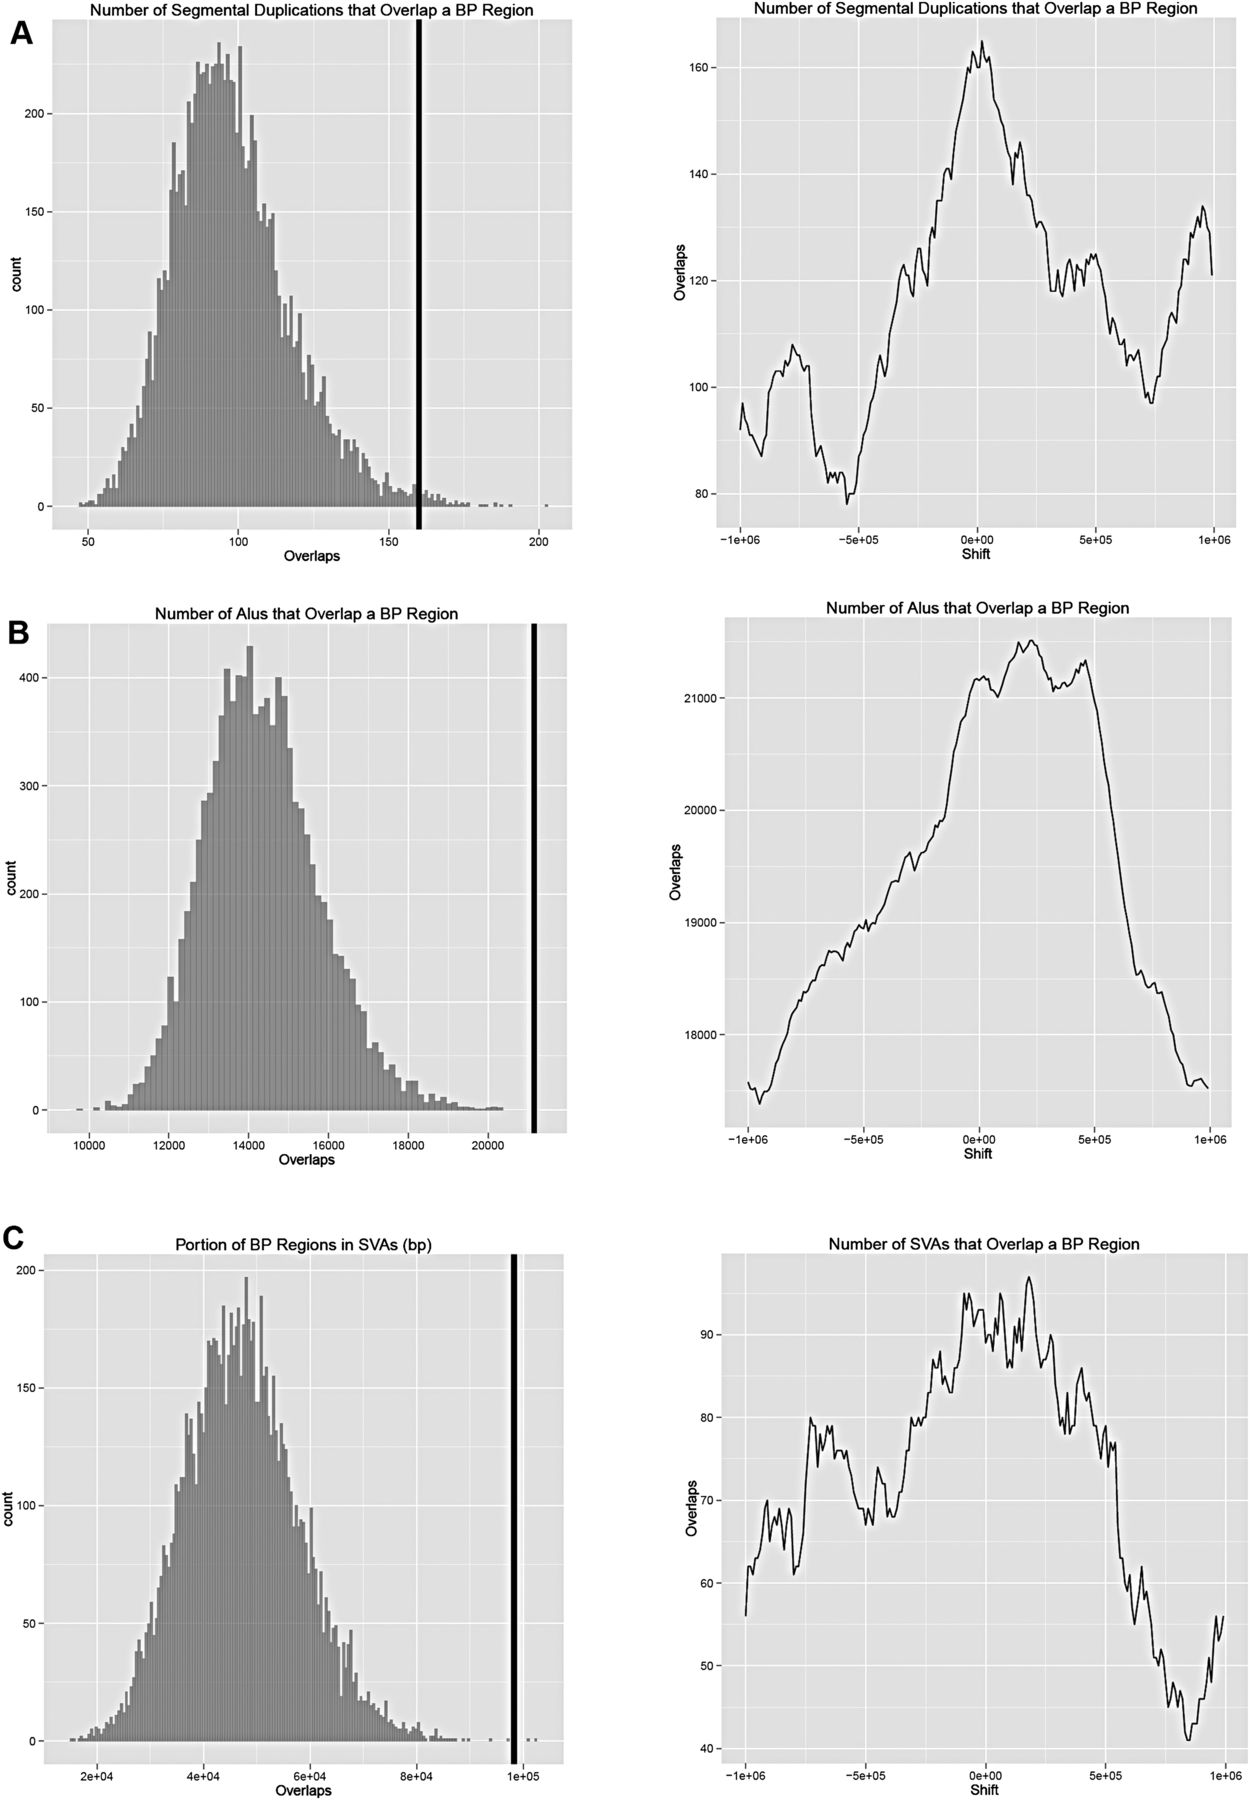
\includegraphics{figures/gibbon_bac_permutations.jpg}
\caption{Enrichment of genomic features in breakpoint regions. Permutation tests were used to assess the overlap between the gibbon breakpoints and genomic features. (A) Segmental duplications; (B) Alu elements; and (C) SVA elements. The black vertical line indicates the observed value for the breakpoints identified in the study. In all three cases it is evident that the genomic features have a higher overlap with the breakpoints than one could expect by chance.}
\label{gibbon_bac_permutations}

\end{figure}

\section{Continuing Analysis of Genomic Breakpoints from Cancer and Evolution}

Continuing the work I have already done in analyzing the evolutionary breakpoints mapped with the gibbon BAC clones, I am working with the International Consortium for Sequencing and Annotation of the gibbon genome to analyze the additional breakpoints discovered through the assembly of the gibbon reference genome. To do so, I am conducting additional association tests with a variety of features. One of these features is a set of binding sites of the evolutionarily conserved binding factor CTCF, which I have identified through the analysis of chromatin immunoprecipitation followed by sequencing (ChIP-seq) data. CTCF has recently been shown to be associated with the three-dimensional structure of DNA and chromatin in the cell~\cite{Dixon:2012gc}, and therefore may have important associations with genomic DNA breakpoints and structural variations.

I am also helping to analyze the breakpoints from a set of over forty mesenchymal tumor samples in which genomic rearrangements have created ring-shaped chromosomes. The breakpoints that cause these chromosomal rearrangements cluster into several frequently broken areas. I am currently working on analyzing these breakpoint regions using my permutation analysis pipeline in order to determine genomic features that may be significantly associated with these breakpoints, including repeat elements, open chromatin sites and other data from ENCODE, and binding motifs for enzymes known to be involved with breakpoint formation.

As part of these analyses I will also explore alternative testing strategies including hypergeometric testing~\cite{Sandve:2013ip} and spatial correlation testing~\cite{Favorov:2012dy}.
